%!TEX root=./thesis.tex

\chapter{Overview}\label{chapter:overview}

In this section, we give a high-level overview of chopped symbolic
execution using the simple program in Figure~\ref{fig:simple}. In
particular, Figure~\ref{fig:simple-main} shows the entry point of the
program (function $\code{main}$), while Figure~\ref{fig:simple-f}
shows the uninteresting code which we would like to skip (function
$\code{f}$).

We start the chopped execution by executing $\code{main}$
symbolically. When a state reaches the function call for $\code{f}$ at
line~\ref{line:call_f}, we create a \textit{snapshot state} by cloning
the current state, and skip the function call. The snapshot state is
shown graphically in Figure~\ref{fig:simple-fig}, where each gray oval
represents a symbolic execution state.

With a snapshot created, we then continue the execution on the current
state, but from this point we must consider that some load
instructions may depend on the \textit{side effects} of the skipped
function~$\code{f}$, \ie the memory locations that $\code{f}$ may
update. 
We compute the side effects of $\code{f}$ using conservative static
\emph{pointer analysis}~\cite{andersen:pointeranalysis, Hind:Paste2001, Smaragdakis:FTPL2015} 
before the symbolic exploration starts, see~\S\ref{chapter:design}.
In our example, the side effects of $\code{f}$ are the memory
locations pointed to by \code{p.x} and \code{p.y}, which are updated
at lines~\ref{line:px_write} and \ref{line:py_write}, respectively.
We define the load instructions that read from memory locations 
which may be updated by skipped functions as \textit{dependent loads}.

On some paths, symbolic execution does not encounter such
\textit{dependent loads}. For example, the path following the
$\code{else}$ side of the branch at line~\ref{line:if_j} accesses
neither \code{p.x} nor \code{p.y}, so no further action is needed on
those paths, and the exploration may correctly terminate without ever
going through the code of $\code{f}$. Indeed, in real programs there
are often paths that do not depend on the skipped functions, and in
such cases symbolic execution immediately benefits from our approach:
irrelevant paths are safely skipped, thus reducing path explosion.

However, on other paths symbolic execution encounters
\textit{dependent loads}.  This happens for our example on the path
which explores the $\code{then}$ side of the branch at
line~\ref{line:if_j}, when it loads the value of \code{p.y} at
line~\ref{line:if_py}. At this point, the current state needs to be
suspended until the relevant paths in function $\code{f}$ are
explored, and becomes a \textit{dependent state}. To recover a path,
we create a new \textit{recovery state} which inherits the snapshot
state generated before skipping $\code{f}$ at line~\ref{line:call_f}
and start executing symbolically the function.

While symbolic execution is in the recovery state, if the execution
forks, then the same fork is performed in the dependent state.
Furthermore, as we run the recovery state, any stores to the memory
location read by the dependent load are also performed in the
dependent state. For example, if the symbolic execution of $\code{f}$
traverses the $\code{else}$ branch at
lines~\ref{line:if_k_else}--\ref{line:py_write}, then the value of
$\code{p.y}$ (the memory location pointed to by $\code{p->y}$) is set
to $1$ in the dependent state too. If the recovery state returns
successfully, the dependent state is resumed successfully. If an error
occurs while executing the recovery state (\eg an invalid memory
access or a division by zero error, which could have occurred if
$\code{p->z}$ were set in line~\ref{line:pz_write} to $\code{4/p->y}$)
the dependent state is terminated.

When we execute a recovery state, not all paths might be compatible
with the execution which the dependent state reached. For example, if
line~\ref{line:if_j} were changed from \code{if (j>0)} to \code{if
  (k>0)}, then the dependent state would have $k>0$ in its path condition, 
which makes the path in $\code{f}$ where $k \le 0$ incompatible.

One way to filter such incompatible paths would be to execute all
possible paths thorough $\code{f}$ during recovery, and later filter
the ones that are incompatible with the dependent state. However, this
would potentially lead to the exploration of a large number of
infeasible paths. We thus designed a more efficient solution: Each
state maintains a list of \textit{guiding constraints}, which are
those constraints added since the call to the skipped function. In our
example, the guiding constraints for the dependent state are
$j>0$. Before we execute a recovery state, we add these
\textit{guiding constraints} from the dependent state to the path
condition of the recovery state. By doing this, we guarantee that
every path explored in the recovery state is consistent with respect
to its dependent state.

During recovery, one could execute all possible paths through the
skipped function $\code{f}$ which are compatible with the dependent
state, as we do in the example above. However, for real programs this
could be unnecessarily expensive, as many paths do not influence the
dependent load which started the recovery. To avoid this possible path
explosion, and reduce the cost of constraint solving, we aim to only
execute the paths that could influence the dependent load. We
accomplish this by statically \emph{slicing}~\cite{Weiser:ICSE1981,
  Tip95asurvey, BinkleyH04, Xu:Slicing2005} the function $\code{f}$
with respect to the store instructions that write to the memory
location read by the dependent load, that is the side effects
observable from the dependent load. Note that function $\code{f}$
could call other functions, so the slicing is done for all these
functions too. In our example, the slicing would likely be able to
completely remove the $\code{if}$ statement at
lines~\ref{line:if_k_z}--\ref{line:pz_write}, which would halve the
number of explored paths, thus reducing path explosion. It would also
likely remove the $\code{then}$ side of the $\code{if}$ statement at
line~\ref{line:if_k}, which in this case does not bring significant
benefits, but it could, if that side of the branch were replaced by
say, an expensive loop. Slicing away these code parts is possible
because they do not update \code{p.y} on which the dependent load on
line~\ref{line:if_py} relies.\footnote{In practice, the success of the
  slicing algorithm in reducing the size of the code depends on the
  precision of the underlying pointer analysis.}

Figure~\ref{fig:simple-fig} shows how chopped symbolic execution works
on our example in a graphical way. To recapitulate, when the call to
$\code{f}$ is reached at line~\ref{line:call_f}, a snapshot state is
created by cloning the current state (step~\step{1} in the figure).
Then, on the execution state that reaches
line~\ref{line:if_py}, the current state becomes a dependent state and
is suspended (step~\step{2}).
A recovery state is created by cloning the snapshot state
and the guiding constraints from the dependent state are added
to the path condition of the newly created recovery state (step~\step{3}).
At this point, function $f$ is statically sliced
where the \textit{slicing criterion} is all the store instructions
which may update \code{p->y} (more specifically, the store at line~\ref{line:py_write}).
In our case, the slicer removes the first \textit{if} statement and the \textit{then} side
of the second \textit{if} statement. Then, the recovery state starts
symbolically executing the sliced version of $\code{f}$.  When execution
is forked at line~\ref{line:if_k}, then the dependent state is also
forked along the same constraints (steps~\step{4} and \step{5}). One
of the forked recovery states (Recovery') updates the location
\code{p->y} on which our dependent load relies on, so this location is
also updated in the corresponding dependent state
(step~\step{6}). Finally, when a recovery state terminates,
it gets discarded  (step~\step{7}), and
symbolic execution is resumed from its dependent states  and other
normal states in the program.

\begin{figure*}[t]
  \centering
  \subfloat[]{
    \lstinputlisting[linewidth=.4\textwidth]{code/simple-main.c}
    \label{fig:simple-main}
  }
  \hspace{30pt}
  \subfloat[]{
    \lstinputlisting[linewidth=.4\textwidth,firstnumber=15]{code/simple-f.c}
    \label{fig:simple-f}
  }
  \hspace{10pt}
  \subfloat[]{
    \raisebox{-100pt}{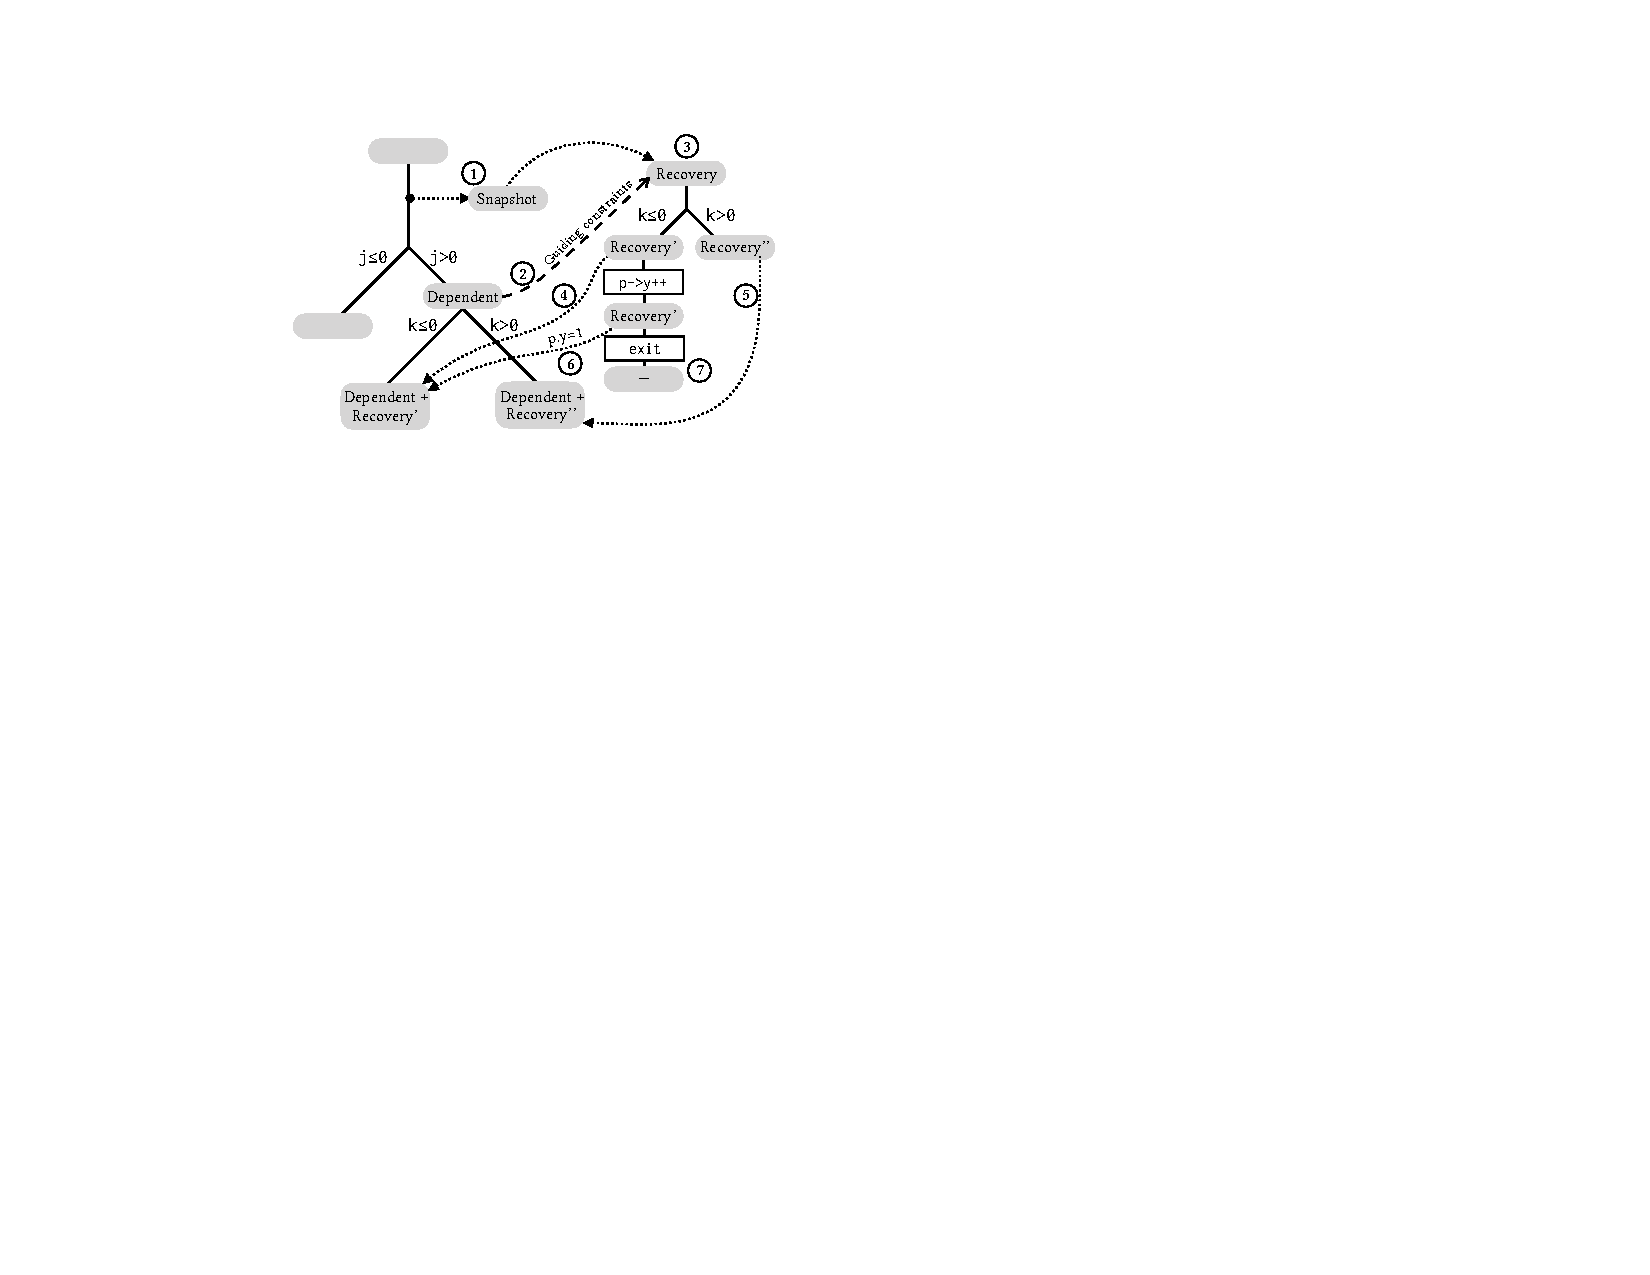
\includegraphics[width=.75\textwidth]{img-states3}}
    \label{fig:simple-fig}
  }
  \caption{Graphical illustration of chopped symbolic execution on a simple example.}
  \label{fig:simple}
\end{figure*}

%% Impact: with this form of symbolic execution we might end up
%% 1- completely skipping some code portions
%% 2- partially skipping some code portions
%% 3- not skipping the irrelevant code portions
%% In cases 2 and 3 we might still drastically reduce the
%% number of program paths and queries to the solver (due to
%% laziness in the evaluation of the skipped code)

%%% Local Variables:
%%% mode: latex
%%% TeX-master: "paper"
%%% End:
